\documentclass[12pt, twoside]{article}
\input{../preamble}

\fancyhead[LO]{La Scuola d'Italia / Dr.\ Huson / IB Math AA SL \\* 13 May 2026}
\fancyhead[RO]{\fbox{\begin{minipage}{4cm}\footnotesize First \& Last name:\\[0.5cm]\end{minipage}}}
\fancyfoot[C]{\thepage}

\begin{document}
\subsubsection*{11.18 Classwork: Series}

Problems 1 and 2 are no calculator. Problems 3 and 4 are calculator allowed.

\begin{enumerate}[itemsep=0.35cm]

%--- Problem 1: Geometric sums and sums of partial sums [5 marks] ---
%--- Source: AA SL 2024 May P1 TZ1 Q6 ---
\item[1.] \makebox[\linewidth][s]{[Maximum mark: 5]\hfill {\small AA SL 2024 May P1 TZ1 Q6}}

Consider a geometric sequence with first term $1$ and common ratio $10$.

$S_n$ is the sum of the first $n$ terms of the sequence.

\begin{enumerate}[itemsep=0.18cm]
  \item Find an expression for $S_n$ in the form
  $\dfrac{a^n-1}{b}$, where $a,b\in\mathbb{Z}^+$. \hfill [1]
  \item Hence, show that
  \[
    S_1+S_2+S_3+\cdots+S_n
    =\frac{10(10^n-1)-9n}{81}.
  \]
  \hfill [4]
\end{enumerate}

\begin{tikzpicture}
  \draw (-0.6,0) rectangle (11,9.5);
  \foreach \y in {1,2,...,9} \draw[dotted] (0,\y)--(10.5,\y);
\end{tikzpicture}

\newpage

%--- Problem 2: Geometric areas, mean, and median [8 marks] ---
%--- Source: AA SL 2025 May P1 TZ1 Q6 ---
\item[2.] \makebox[\linewidth][s]{[Maximum mark: 8]\hfill {\small AA SL 2025 May P1 TZ1 Q6 (no calculator)}}

Consider a sequence of ten rectangular picture frames
$F_1,F_2,\ldots,F_9,F_{10}$.

Picture frame $F_1$ has width $4\text{ cm}$ and height $5\text{ cm}$.

The width and height of picture frame $F_n$ are each increased by $50\%$
to generate the width and height of the next picture frame $F_{n+1}$, for
$n\in\mathbb{Z}^+$, $1\leq n\leq 9$.

\begin{enumerate}[itemsep=0.18cm]
  \item \begin{enumerate}[itemsep=0.12cm]
    \item[(i)] Show that the area of picture frame $F_n$ is
    $20\left(\frac{9}{4}\right)^{n-1}\text{ cm}^2$. \hfill [2]
    \item[(ii)] Hence, find the mean area of the ten picture frames,
    giving your answer in the form
    $p\left(\left(\frac{9}{4}\right)^a-1\right)\text{ cm}^2$,
    where $p\in\mathbb{Q}^+$ and $a\in\mathbb{Z}^+$. \hfill [3]
  \end{enumerate}
  \item Find the median area of the ten picture frames, giving your
  answer in the form $q\left(\frac{9}{4}\right)^4\text{ cm}^2$,
  where $q\in\mathbb{Q}^+$. \hfill [3]
\end{enumerate}

\begin{tikzpicture}
  \draw (-0.6,0) rectangle (11,8.2);
  \foreach \y in {1,2,...,8} \draw[dotted] (0,\y)--(10.5,\y);
\end{tikzpicture}

\newpage

%--- Problem 3: Card pyramids and arithmetic sums [16 marks] ---
%--- Source: AA SL 2025 May P2 TZ1 Q8 ---
\item[3.] \makebox[\linewidth][s]{[Maximum mark: 16]\hfill {\small AA SL 2025 May P2 TZ1 Q8}}

Rectangular playing cards are stacked in the shape of a pyramid with $n$
rows, where $n\geq 1$.

Some cards are placed horizontally and some cards are stacked at an angle
of $60^\circ$ to the horizontal.

The following diagrams represent pyramid stacks for $n=1$, $n=2$ and
$n=3$.

\begin{center}
  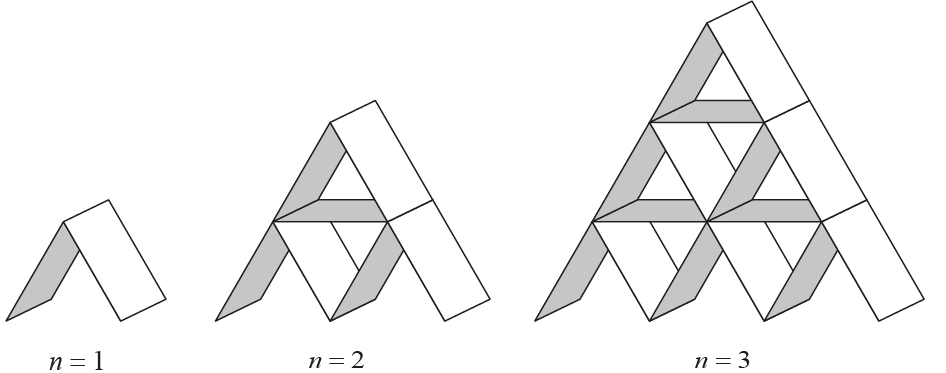
\includegraphics[width=0.72\textwidth]{../graphics/series-card-stacks.png}
\end{center}

Let $t_n$ represent the number of cards used to create a pyramid stack
with $n$ rows.

\begin{enumerate}[itemsep=0.10cm]
  \item Write down $t_3$. \hfill [1]
  \item Find $t_4$. \hfill [2]
  \item Show that \hfill [3]
  \[
    t_n=\frac{n(3n+1)}{2}.
  \]
\end{enumerate}

There are $52$ cards in a full pack of playing cards.

\begin{enumerate}[itemsep=0.10cm]
  \item[(d)] A complete pyramid stack is created using playing cards
  taken from $14$ full packs. Find the maximum number of rows in this
  stack. \hfill [3]
  \item[(e)] A complete pyramid stack is created using playing cards
  taken from full packs with no cards left over. Find the minimum number
  of rows in this stack. \hfill [2]
\end{enumerate}

The long edge of each playing card measures $88\text{ mm}$ as illustrated
in the following diagram.

\begin{center}
  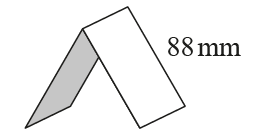
\includegraphics[width=0.23\textwidth]{../graphics/series-card-edge.png}
\end{center}

\begin{enumerate}[itemsep=0.10cm]
  \item[(f)] Find the minimum number of cards needed to create a complete
  pyramid stack with a vertical height of more than $2$ metres. The
  thickness of the cards may be ignored. \hfill [5]
\end{enumerate}

\newpage

%--- Problem 4: Simple and compound interest comparison [12 marks] ---
%--- Source: AA SL 2025 Nov P2 TZ3 Q7 ---
\item[4.] \makebox[\linewidth][s]{[Maximum mark: 12]\hfill {\small AA SL 2025 Nov P2 TZ3 Q7}}

Andy and Jess each have $\$5000$.

Andy invests the money in a new savings plan that will pay interest at
the end of each month.

Andy will receive a fixed amount of interest each month. The amount
received is $0.315\%$ of the initial investment.

\begin{enumerate}[itemsep=0.18cm]
  \item \begin{enumerate}[itemsep=0.12cm]
    \item[(i)] Determine the amount of interest Andy will receive at the
    end of each month. Give this answer correct to two decimal places.
    \hfill [1]
    \item[(ii)] Hence, determine the amount of interest Andy will receive
    each year. \hfill [1]
    \item[(iii)] Write down an expression in the form $5000+pn$, where
    $p\in\mathbb{Z}^+$, for the amount of money Andy will have in his
    savings plan at the end of $n$ years. \hfill [1]
    \item[(iv)] Hence, show that Andy will have $\$5945$ in his savings
    plan at the end of $5$ years. \hfill [1]
  \end{enumerate}
\end{enumerate}

In this part, where appropriate, give all answers to the nearest dollar.

Jess invests her $\$5000$ in a new account that pays $3\%$ interest
compounded annually.

\begin{enumerate}[itemsep=0.18cm]
  \item[(b)] \begin{enumerate}[itemsep=0.12cm]
    \item[(i)] Determine the amount of money that will be in Jess's
    account at the end of $5$ years. \hfill [2]
    \item[(ii)] Hence, find the amount of interest Jess will receive in
    the $5$ years. \hfill [1]
  \end{enumerate}
  \item[(c)] \begin{enumerate}[itemsep=0.12cm]
    \item[(i)] Write an expression in the form $5000\times q^n$, where
    $q\in\mathbb{R}^+$, for the amount of money that Jess will have in
    her account at the end of $n$ years. \hfill [2]
    \item[(ii)] Hence, determine the smallest number of complete years
    that it will take for Jess to have more money in her account than
    Andy has in his savings plan. \hfill [3]
  \end{enumerate}
\end{enumerate}

\end{enumerate}
\end{document}
